\documentclass[onecolumn, draftclsnofoot, 10pt, compsoc]{IEEEtran}
\usepackage{graphicx}
\graphicspath{{./figures/}}

\usepackage{url}
\usepackage{setspace}
\usepackage{multicol}
\usepackage{pdflscape}
\usepackage{pdfpages}
\usepackage{caption}

\usepackage{geometry}
\geometry{textheight=9.5in, textwidth=7in}

\renewcommand\refname{}

\usepackage[numbers]{natbib}
\bibliographystyle{IEEEtranN}

% \overfullrule=2in

% 1. Fill in these details
\def \CapstoneTeamName{			Ground Station Software Team}
\def \CapstoneTeamNumber{		30}
\def \GroupMemberOne{			Kenneth Steinfeldt}
\def \GroupMemberTwo{			Christopher Pham}
\def \GroupMemberThree{			Corwin Perren}
\def \CapstoneProjectName{		OSU Robotics Club\\Mars Rover Ground Station}
\def \CapstoneSponsorCompany{	OSU Robotics Club}
\def \CapstoneSponsorPerson{	Nick McComb}


% 2. Uncomment the appropriate line below so that the document type works
\def \DocType{	%Problem Statement
				%Requirements Document
				%Technology Review
				Design Document
				%Progress Report
			 }
			
\newcommand{\NameSigPair}[1]{
  \par
  \makebox[2.75in][r]{#1} 
  \hfill
  \makebox[3.25in]{
      \makebox[2.25in]{\hrulefill} 
      \hfill
      \makebox[.75in]{\hrulefill}
  }
  \par\vspace{-12pt} 
  \textit{
      \tiny\noindent
      \makebox[2.75in]{} 
      \hfill
      \makebox[3.25in]{
          \makebox[2.25in][r]{Signature} 
          \hfill
          \makebox[.75in][r]{Date}
      }
  }
}
% 3. If the document is not to be signed, uncomment the command below
\renewcommand{\NameSigPair}[1]{#1}

%%%%%%%%%%%%%%%%%%%%%%%%%%%%%%%%%%%%%%%
\begin{document}
\begin{titlepage}
	\pagenumbering{gobble}
	\begin{singlespace}
		% 4. If you have a logo, use this includegraphics command to put it on the coversheet.
        \begin{minipage}{7in}
			\centering
			\hspace*{-.7in}
			$\vcenter{\hbox{
\includegraphics[height=4cm]{Oregon_State_College_of_Engineering_Logo}}}$
			\hspace*{.2in}
			$\vcenter{\hbox{
\includegraphics[height=2.5cm]{OSURCLogoOrange}}}$
		\end{minipage}

		\par\vspace{.35in}
		\centering
		\scshape{
			\huge CS Capstone \DocType \par
			{\large\today}\par
			\vspace{.5in}
			\textbf{\Huge\CapstoneProjectName}\par
			\vfill
			{\large Prepared for}\par
			\Huge \CapstoneSponsorCompany\par
			\vspace{5pt}
			{\Large\NameSigPair{\CapstoneSponsorPerson}\par}
			{\large Prepared by }\par
			Group\CapstoneTeamNumber\par
			% 5. comment out the line below this one if you do not wish to name your team
			\CapstoneTeamName\par 
			\vspace{5pt}
			{\Large
				\NameSigPair{\GroupMemberOne}\par
				\NameSigPair{\GroupMemberTwo}\par
				\NameSigPair{\GroupMemberThree}\par
			}
			\vspace{20pt}
            \begin{abstract}
			% 6. Fill in your abstract
            This document describes the design of the Mars Rover Ground Control software for the purpose of conveying design decisions and information to the project's stakeholders.
            The Software Design Description (SDD) supplies a clear picture of the software's future implementation and provides the development group with a clear road-map.

		\end{abstract}
		}
	\end{singlespace}
\end{titlepage}
\newpage
\pagenumbering{arabic}
\tableofcontents
\clearpage

% Major requirements per website:
% - Each member writes up three pieces they will be owning/managing
% - Full document still needs an intro and conclusion
% - This is a HOW document (finally). Can contain info like:
% -- APIs
% -- Time-line
% -- Testing Information
% - Document must follow IEEE Std 10-16-2009 structure
% - Each component design pieces must be at least 500 words
% - Full doc must be at least 1500 words (literally impossible to NOT hit XD)
% - Must use IEEEtran numbered citations
\section{Introduction}\subsection{Purpose}
The purpose of this software design document is to cover the design for the Oregon State University Mars Rover Team's ground station software.
It will cover the details about how the software will function, how we will implement that functionality, and the reasoning behind design decision choices that were made.
The ground station software for the Mars Rover project is the single point of contact between the team-built competition Rover and the users operating or viewing the rover.


\subsection{Scope}
This project will consist of a software package running from a remote control base station in order to remotely operate a competition-ready robot built by the Oregon State Robotics Club's Mars Rover team.
The project must be completed by May 31st 2018 in order to be ready for the University Rover Challenge taking place in Hanksville, Utah.
The controlling software must be able to do at minimum, the following: 

\begin{itemize}
\item Provide the capability to remotely drive the Rover via joysticks connected to the ground station computer.
\item Allow for viewing of up to three video feeds from the Rover, and be able to change what video streams are viewed.
\item Via a user input device, allow for manipulation of the Rover arm.
\item Provide visual feedback about the state of the joint positions of the arm as it is being moved.
\item Show the user a map of the competition area, allowing the user to zoom, view the Rover's location, and place navigation and landmark way-points.
\item Allow the user to add way-points and then place the Rover in autonomous mode, wherein the Rover will drive under its own control along the way-points provided.
\item Upon completion of an autonomous path, provide an easy to read notification that the navigation is complete.
\item Provide a myriad of status information about the Rover's current condition including, but not limited to, the following:
  \begin{itemize}
  \item Connection statuses
  \item Rover Sub-system connection statuses
  \item On-board sensor readings
  \item Battery charge level
  \item System Errors
  \end{itemize}
\item Include documentation allowing for easy reuse of the software for future Rover competition years.
\end{itemize}

Additionally, the client has requested a document be written providing a starting guide on how to re-use the finalized software package for future Rover teams to ease development in future years.


\subsection{Context}
Each year the Mars Rover software team writes ground station software from scratch in order to meet the changing requirements of both the Rover itself and competition rule changes.
As this software is the main point of contact between the users and the Rover, the success of the team during competition often hinges on how well this software performs.
In the past, lack of modularity and abstraction has made re-use of the ground station code near impossible.


\subsection{Summary}
This rest of this document will provide the details about how our team will implement the ground station software for the Mars Rover team.
We will start by covering design considerations such as the environment our software will be running in, as well as the specific concerns of our stakeholder. 
Immediately following will be a breakdown of the individual software components we will be writing.
These will include descriptions of what, how, and why we will be writing each component the way we are.
The document ends with a visual breakdown of the software UI, and rationale for why each component looks the way it does.
\section{References}\vspace{-2em}
\bibliography{bibliography}
\section{Glossary}\subsection{Acronyms and Abbreviations}
\begin{itemize}
\item ROS - Robot Operating System
\item GPS - Global Positioning Satellite
\item OSU - Oregon State University
\item OSURC - Oregon State University Robotics Club
\item NASA - The National Aeronautics and Space Administration
\end{itemize}


\subsection{Definitions}
\begin{itemize}
\item Ubuntu - A popular open source Linux distribution based on the classic Debian distribution.
\item Rover - A robotic, remote controlled vehicle designed and built by OSURC to compete in the NASA Mars Rover Competition held in Hanksville, Utah.
\item QT - An open source application framework developed by the QT Company.
\item Python - A popular scripting language known for it's easy readability and rapid deployment abilities.
\end{itemize}
\section{Design Considerations}\subsection{Assumptions}
From the descriptions and restrictions provided by the client, there are a few things that we need to assume to assure that the software will function correctly. 
Our team is going to assume that the software/OS on the rover is going to be a combination of ROS Kinetic on Ubuntu 16.04. 
The rover will have all of its components working correctly such as GPS and drive systems.
The rover needs to correctly interact with the data that is provided by the station. 
The rover needs to be connected to the same network as the rover.


\subsection{General Constraints}
\begin{itemize}
\item \textit{Time Frame:} The software must be completed on or before May 31st, 2018.
\item \textit{URC Requirements:} The software must not violate any rules provided by the competition host. \cite{urc_competition_rules}
\end{itemize}


\subsection{System Environment}
\begin{itemize}
\item Hardware
  \begin{itemize}
  \item 1 x Intel NUC
  \item 2 x 24" 1080p Monitors
  \item 1 x Keyboard
  \item 1 x Mouse
  \item 1-2 x USB Joystick
  \item 1 x SpaceMouse Pro
  \item 1 x Ubiquiti Rocket M2 Wireless Router
  \end{itemize}
\item Software / OS / Libraries
  \begin{itemize}
  \item Ubuntu 16.04 LTS
  \item ROS Kinetic
  \item Python 2.7
  \item Additional Python Libraries
    \begin{itemize}
    \item PyQt5
    \item inputs
    \item PyGame
    \item spnav
    \item cv2
    \item Pillow
    \item qimage2ndarray
    \end{itemize}
  \end{itemize}
\end{itemize}


\subsection{Stakeholder Concerns}
\subsubsection{Reliability}
The ground control software must be as reliable as possible.
The rover operator must be able to complete all competition tasks, assuming all hardware on the Rover is functioning properly.
If unable to do so, the software cannot be considered a success.
\subsubsection{Robustness}
The University Rover Challenge requires that the rover operate successfully in a variety of environments.
For example, it is expected that as the rover advances through the course, range and obstacles will negatively effect the latency and bandwidth of the wireless Ethernet connection used to communicate with the rover.
In the above example, the rover must be able to downgrade the video feed in order to accommodate the lowered communication abilities of the rover.
\subsubsection{Rapid Prototyping}
In order to fulfill the necessary reliability and robustness requirements of the client, the team must be able to rapidly prototype the software.
Rapid prototyping allows the team to maximize testing time.
\subsubsection{Documentation}
The client has requested that documentation be a primary concern of the project.
The ground control software will be used as a foundation for future rover competitions, therefore it is important that the software is easy to use and the code is easy to understand.
\section{Component Design}\subsection{Human Interface Device Integration}
\subsubsection{Overview}
During use of this ground station software, the user will need to be able to interact with a joystick(s) and SpaceNav mouse to control ground station software elements, to drive the Rover, and to manipulate the Rover arm.
The systems that integrate with these HID devices will be some of the most active parts of the ground station software.

\subsubsection{Design Concerns}
\begin{itemize}
\item \textit{Control Latency:} Latency for these control inputs must be kept to a minimum to ensure that the Rover responds quickly to control commands and that motion is fluid.
\item \textit{Reliability:} As these control inputs can directly control the Rover, the code must be reliable, robust, and be able to recover from errors such as a disconnect and reconnect of a joystick.
\item \textit{Flexibility:} It is hard to determine the best possible control scheme for the Rover via these control inputs until the team has had a chance to physically drive the robot, so having the flexibility to easily change the control structure is important.
Additionally, these input devices may change completely if they are determined to be inadequate in real-world tests later on.
\end{itemize}

\subsubsection{Design Elements}
\begin{itemize}
\item The HID integrators will use the \texttt{inputs} or \texttt{pygame} libraries for joysticks or the \texttt{spnav} library for the SpaceNav mouse.
\item Each integrator will be housed within a QThread class that will monitor the state of the HID devices and poll the devices for changes.
\item Upon a device change, the class will broadcast the updates using QSignals so that other parts of the program may use the data.
\item Upon an HID failure, such as on accidental disconnect, the class will attempt to reconnect and broadcast an error state until it is resolved.
\end{itemize}

\subsubsection{Design Rationale}
One of the main goals of this project is to be able to rapidly prototype the software so the Rover team can spend more time testing, and less time waiting for code to be written.
By using off the shelf libraries for reading in joystick and SpaceNav mouse input, our team's development time can be better put to use making the control systems robust and handling error cases.
As these are commonly used and tested libraries, there is also a high likelihood that their implementations are more reliable and documented than if our design team were to try and implement equivalent libraries/classes ourselves.
The use of QT's QSignals will also help us in this regard by minimizing the design time needed to write custom inter-thread communication protocols. 
\subsection{Drive Coordinator - NOT AT WORD COUNT XXX/500}
\subsubsection{Overview}
This sub-system will handle taking in raw joystick/s control information, and transforming them into usable drive control commands.
This will also handling the interpretation of button presses on the joystick to control GUI functions, or for example, artificially limiting the Rover max speed via the current state of the joystick throttle lever.

\subsubsection{Design Concerns}
\begin{itemize}
\item \textit{:} REPLACE

\end{itemize}

\subsubsection{Design Elements}
\begin{itemize}
\item REPLACE
\end{itemize}

\subsubsection{Design Rationale}

\subsection{Mapping System - NOT AT WORD COUNT 410/500}
\subsubsection{Overview}
The mapping sub-system will handle the storing and loading of maps of the competition area as well as plotting important landmarks as provided by the user.

\subsubsection{Design Concerns}
\begin{itemize}
\item \textit{Offline Use:} As this software will primarily be used in environments where there are no Internet connections, the mapping sub-system will need to be able to store local maps of the desired competition areas in advance.
\item \textit{Zoom Options:} During competition, the user may desire to zoom in or out on any particular area. 
The software will have to accommodate this by either digitally zooming into an the desired area, or by loading newer high-resolution images at a adjusted zoom level.
\item \textit{Location Services:} The mapping system must accurately show where the rover is on the map so that the operator is able to keep track of it.
Furthermore the mapping must also allow the setting of waypoints.
These waypoints allow the operator to set a location that the rover will travel to once set.
\item \textit{Reliability:} The mapping system will be one of the most used aspects of the ground station software as it will be used for properly navigating the Rover to competition way-points. 
If the mapping system fails, it may be near impossible for the user to determine where the Rover should be driven.
\item \textit{Responsiveness:} Outside of the drive and video sub-systems, the mapping system will be one of the most frequently updated and used features on the ground station software.
In order for it to be useful to the user the map updates must be fast and responsive so that the user is not spending valuable competition time waiting for the map to load.
\end{itemize}

\subsubsection{Design Elements}
\begin{itemize}
\item The mapping system will load satellite imagery of the desired area via the Google Maps API.
\item The Google Maps tiles will be cached so they can be used offline.
\item Individual image tiles will be stitched together into one large image to be shown in the GUI using either OpenCV or Pillow.
\item The map will have icons and/or numbers overlaid on the map image corresponding to the Rover location, navigation way-points, and landmark way-points.
\item The aforementioned markers will be accurate on the map based on their GPS positions.
\item The map will show a trail of the Rover's previous driving path that fades away over time.
\item The map will have a faint grid showing latitudinal and longitudinal divisions.
\end{itemize}

\subsubsection{Design Rationale}
The choice of the Google Maps API allows us to use the most up-to-date and readily available maps of the competition area easily.
OpenCV and Pillow are both fast and well-documented frameworks for dealing with image data, and are especially good at fast image stitching.
The other design aspects of the mapping system should make the map view easy and intuitive to use, meaning less training will be necessary before a user will understand it.
\subsection{Way-points Coordinator - NOT AT WORD COUNT XXX/500}
\subsubsection{Overview}

\subsubsection{Design Concerns}
\begin{itemize}
\item \textit{REPLACE:} REPLACE

\end{itemize}

\subsubsection{Design Elements}
\begin{itemize}
\item REPLACE
\end{itemize}

\subsubsection{Design Rationale}

\subsection{Arm Visualizer}
\subsubsection{Overview}
The arm visualizer will allow the user to quickly and easily view and understand where the joints on the Mars Rover arm are at any given time.
As the arm is moved, these visual indicators will update to show the new arm positions.

\subsubsection{Design Concerns}
\begin{itemize}
\item \textit{Viewing Simplicity:} The indicators need to be visually displayed in such a way that the user instinctively understands what the data means.
\item \textit{Responsiveness:} In order to be useful, the indicators will need to update quickly.
During competition, the user will use these indicators to position the arm, and major delays in updating these will make them unpleasant to use.
\item \textit{Clutter:} As there are many competition events where the arm will not be needed, these visualizations should be able to be disabled so that there is not unnecessary clutter and information on-screen when it is not needed.
\end{itemize}

\subsubsection{Design Elements}
\begin{itemize}
\item The arm visualizer will take in position information via a ROS topic using \texttt{rospy}.
\item The arm visualizer will, in the initial version, show this information in native QT GUI elements such as a QGraphicsView or QPixmap embedded in a QLabel.
\item The arm visualizer will black out the unneeded visual elements when the arm is not presently attached to the Rover.
\item In the event there is spare time, the previous visualizations will be replaced with a 3D visualization of the Rover through ROS' RVIZ tool, where the position changes accurately correspond to movement changes on the model. 
\item If the previous option is not attainable, the visualizer will attempt to be replaced with a custom OpenGL widget containing the 3D view of the Rover arm, and like previously, will update the model to match the current arm position.
\end{itemize}

\subsubsection{Design Rationale}
By taking in position information through ROS topics with \texttt{rospy}, we will be able to avoid having to write a custom network message system to provide and interpret this data from the Rover, which would have been a tedious and error prone process.
Using native QT widgets, at least for the initial version, will mean that we can more quickly get the pertinent information into a display format that can be understood. 
The QGraphics view widget in particular will let us draw a scene in a painting environment, and then manipulate the scene to show a arrow moving around a circle for example, with relative ease.

\subsection{Arm Coordinator - NOT AT WORD COUNT XXX/500}
\subsubsection{Overview}

\subsubsection{Design Concerns}
\begin{itemize}
\item \textit{REPLACE:} REPLACE

\end{itemize}

\subsubsection{Design Elements}
\begin{itemize}
\item REPLACE
\end{itemize}

\subsubsection{Design Rationale}

\subsection{Video Coordinator}
\subsubsection{Overview}
The video coordinator will handle taking in video stream data from the Rover, and displaying that data on the GUI.
It will also handling telling the Rover what resolution and potentially bit-rate the ground station would like from a particular camera.
Lastly, it will handle switching which video streams are showed in each of the three video display areas on the GUI, including the ability to switch off the secondary/tertiary displays.

\subsubsection{Design Concerns}
\begin{itemize}
\item \textit{Reliability:} The live video streams are a necessity to be able to remotely operate the Rover for most competition events. 
If the video streams are not functioning, the Rover will do very poorly in competition.
\item \textit{Processing Time:} As the video streams will be used the drive the Rover remotely, processing delays should be kept to an absolute minimum so that the driving experience feels more fluid.
\item \textit{Resolution Change Detection:} The user should not have to manually change resolutions if a video that was on the primary video window is switched to the secondary or tertiary window.
This does not apply if the user overrides the resolution settings in order to get smoother video during times of poor radio reception.
\end{itemize}

\subsubsection{Design Elements}
\begin{itemize}
\item The video coordinator will use \texttt{rospy} to retrieve compressed video data streams from the Rover.
\item The video coordinator will format the video data in a way that it can be displayed on a QLabel as an embedded QPixmap.
\item The video coordinator will automatically send resolution adjustment commands to the Rover over a ROS topic as the video streams are switched between the primary and secondary/tertiary video windows.
\item The video coordinator will automatically handle adjusting the video data so it can be properly shown in the QLabel, even after a resolution adjustment.
\item The video coordinator will handling blanking out the secondary/tertiary video displays and stop processing the underlying video if a user requests it.
\end{itemize}

\subsubsection{Design Rationale}
By using ROS' built-in compressed video streams, and the accompanying \texttt{rospy} libraries for interpreting this video data, our team can focus on the logistics of showing these videos on the GUI.
By handling automatic resolution adjustment, we are simplifying the tasks the user will have to perform during competition.
The automatic adjustments also help alleviate unnecessary network bandwidth for streams that would not benefit from the higher resolution. 
Automatic adjustments will both lower latency and allow the Rover to have to process less data, which are both positives in a remote, battery-powered environment.

\subsection{Statuses Coordinator}
\subsubsection{Overview}
The statuses coordinator will be tasked with handling all the miscellaneous messages being sent to the ground station from the Rover.
It will take in these messages and route them to GUI elements for display.
This will include information such as Rover battery level, raw GPS data for the mapping sub-system, and whether sub-components of the Rover are connected, such as the arm.

\subsubsection{Design Concerns}
\begin{itemize}
\item \textit{Minimal Overhead:} As most of these messages are non-critical, it is important for this coordinator to keep its resource usage low so that the processing power is available for other ground station functions.
\item \textit{Fast Navigational Updates:} Since navigational updates will be part of these messages, it will be important for these messages to be prioritized for updates to GUI elements such as the compass and speed indicators.
\item \textit{Adequate Warnings:} It will be important that this coordinator provides noticeable warnings, potentially through methods such as flashing indicators, when there are problems with Rover systems that it has received a message about.
Depending on the warning, a low battery for example, it could be the difference between the Rover winning or losing a competition event.
\end{itemize}

\subsubsection{Design Elements}
\begin{itemize}
\item The statuses coordinator will take in Rover status messages via ROS topics using \texttt{rospy}.
\item The statuses coordinator will update any necessary GUI elements such as QLabels with their pertinent formatted information as received via the ROS messages.
\item The statuses coordinator will prioritize any updates to GPS and navigation messages so that the user can more easily drive the Rover.
\item The statuses coordinator will brightly flash GUI elements that it feels the user needs to pay attention to, and allow the user to cancel the warning by clicking on the GUI element.
\end{itemize}

\subsubsection{Design Rationale}
By using ROS topics to handle messages from the Rover to the GUI, our team is able to spend that time working on quickly showing these updates instead of creating custom network message protocols.
Prioritizing updates to the navigation GUI elements when performing updates will help the user driving the Rover more reliably understand what the Rover is doing movement-wise, which is more important than secondarily important messages such as battery voltage.
By flashing GUI elements in bright colors, and allowing users to cancel these warnings, we are bringing the proper amount of attention to messages that need it while not being obnoxious and having these warning continue indefinitely.

\subsection{Logging / Recording Coordinator}
\subsubsection{Overview}
Recording and logging information is very important for monitoring the rover's status and re-run how a rover was performing during some set period.

\subsubsection{Design Concerns}
\begin{itemize}
\item \textit{Storage Space:} With all the video/recording the system is going to do, the space might be limited on the system or on the rover.
\item \textit{Video Bitrate:} The video should be recorded in a quality that is independent of the streaming video stream to allow full video quality when retrieved
\item \textit{Storage Format:} With the variable size of log files, some settings might be necessary to control logging location, size, or type. 
\end{itemize}

\subsubsection{Design Elements}
\begin{itemize}
\item The coordinator will take any information from the rover as a stream of information.
\item The coordinator will store any video stream that the rover sends back to save back on overhead on the rover.
\item The rover will not be saving any files to allow for overhead and processing.
\end{itemize}

\subsubsection{Design Rationale}
The rover is going to be overloaded with calculations and trans-coding, so the ground station should be able to offload any extra computation onto it.
The ground control system will take care of storing information like log files in session logs.
There is an inbuilt system using ROS that makes a bag that can be used to log everything.









\section{User Interface Design}\subsection{Left Screen}
\subsubsection{Mock-up}
\vspace{1em}
\begin{minipage}{\linewidth}
  \begin{center}
  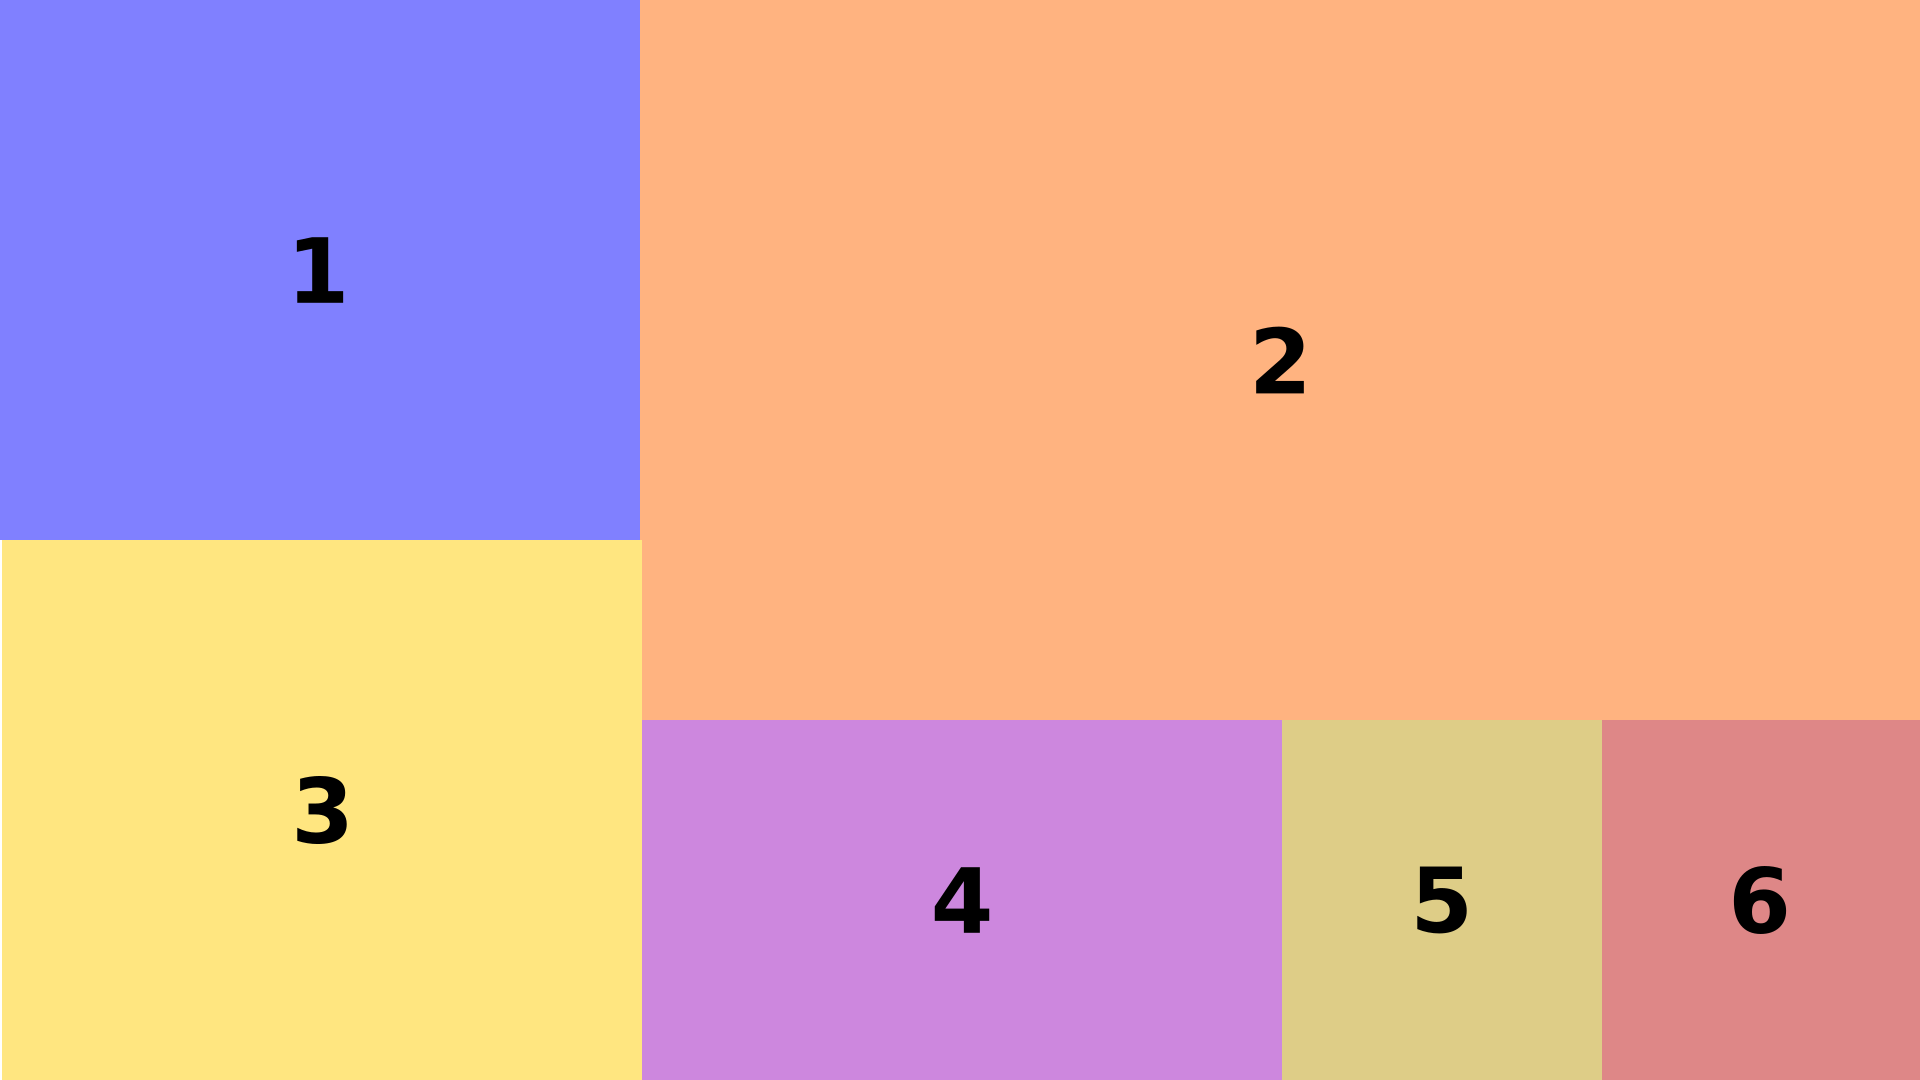
\includegraphics[width=0.75\linewidth]{left_screen_svg}
  \captionof{figure}{Left Screen Mock-up}
  \end{center}
\end{minipage}

\subsection{Zones}
\subsubsection{1: System Statuses / Sensor Readings}
This section will display all status and sensor data both from the Rover and about the ground station itself.
This includes items such as radio signal strength, GPS accuracy, and whether they Ground Station has connection to the drive joystick/s and SpaceNav mouse.

\subsubsection{2: Map Display}
The map display will display a satellite view of the competition areas with navigation and land-mark way-points, the Rover, and the Rover movement trail overlaid.

\subsubsection{3: Recording / Logging / Settings}
This section will be tabbed group that by default will show the controls for starting ROS bag recordings, but will also have a tab for live logs and a third tab for settings to adjusting items such as what map is being shown.

\subsubsection{4: Way-point Entry / Autonomy Controls}
This block will also for manual entry of GPS coordinates, as are provided by the competition at the beginning of some events.
The user will be able to chose whether the entry is being added as a navigation or landmark way-point as well as using the entry fields to edit the way-points from pre-entered points.


\subsubsection{5: Navigation Way-points Listing}
This area will list, in order, the navigation way-points that the system is currently set to follow, both for manual driving and for the autonomy portion.

\subsubsection{6: Landmark Way-points Listing}
This will list, in the order they were added, the landmark way-points that the user has entered to make important points on the competition field.

\subsection{Layout Rationale}
This display shows most of the information regarding the Rover that does not need to be viewed while the Rover is being actively driven, or while the arm is being moved.
When the software starts and is first connecting to the Rover, the user will spend some time studying system statuses, entering way-points, changing settings, and checking logs if needed.
Once they're done with these initial checks and entries, most of the rest of the control experience will take place on the right hand monitor.
In the case that the user wants to quickly glance at the map while they are driving, the map will come in to view easily as it's as close to the right hand monitor as it can be.
As the logging and setting views will hopefully not need to be viewed very often, combining them onto a tabbed GUI element helps reduce used space while still leaving them accessible when needed.


\subsection{Right Screen}
\subsubsection{Mock-up}
\vspace{1em}
\begin{minipage}{\linewidth}
  \begin{center}
  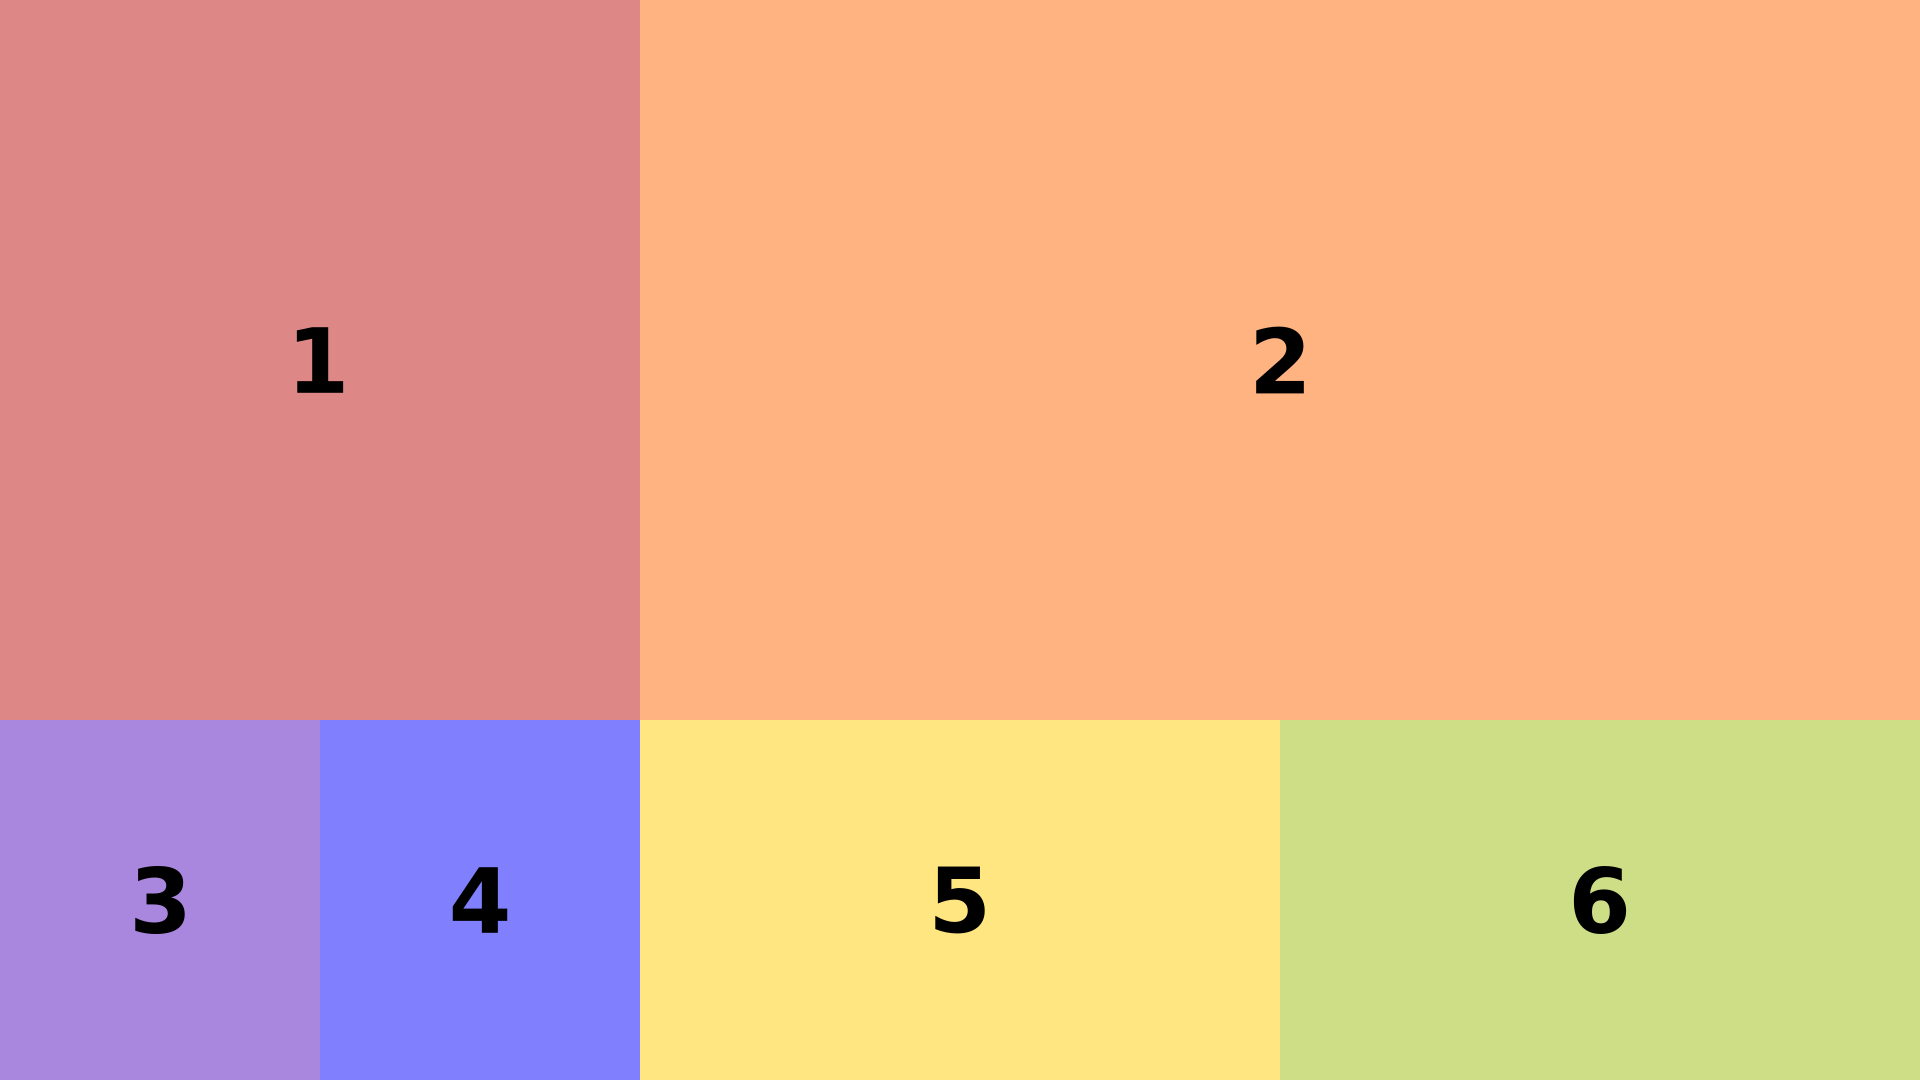
\includegraphics[width=0.75\linewidth]{right_screen_svg}
  \captionof{figure}{Right Screen Mock-up}
  \end{center}
\end{minipage}

\subsection{Zones}
\subsubsection{1: Arm Visualization}
This visualization area will show the joint positions of the Rover arm when the arm is attached.
In its simplest form, the visualization will be a simple line drawn in a reference frame, that adjusts its position as the arm is moved.
For this version, each joint would have its own visualization box.
If there is enough time, our team will attempt to integrate with RVIZ, the ROS visualization package, to show a 3D view of the arm moving.
If the RVIZ solution does not seem feasible and there is still extra time, we may alternatively try to implement a custom OpenGL view of the arm.

\subsubsection{2: Primary Video Display}
This will show the stream from the camera on the Rover is currently selected as the primary video stream.


\subsubsection{3: Heading Compass}
This heading compass will dynamically rotate to match the current heading of the Rover.
It will also mark on the compass edge the currently active way-point, making it easy for the user driving the Rover to determine which direction they need to turn to line up with a way-point marker.


\subsubsection{4: Speed and Speed Limit Display}
This area will show the current Rover speed is meters per second as is reported by the Rover GPS.
Additionally, it will also show the current speed limit of the Rover from zero to one hundred percent as has been limited by the user via the joystick throttle lever.


\subsubsection{5: Secondary Video Display}
This area will show the stream from the camera on th Rover that is currently selected as the secondary video stream.
This stream has the capability to be disabled and show a placeholder image if the team needs to save on radio bandwidth.


\subsubsection{6: Tertiary Video Display}
This area will show the stream from the camera on th Rover that is currently selected as the tertiary video stream.
This stream has the capability to be disabled and show a placeholder image if the team needs to save on radio bandwidth.


\subsection{Layout Rationale}
This screen will be showing the most commonly looked at data for the user driving the Rover.
During a normal competition, the user will start by entering way-points to drive the Rover to, and then switch to the joystick and SpaceNav mouse.
Once they start driving, the user will be heavily focused on monitoring video data to make sure they don not run the Rover into anything. 
While driving to the way-points to get to an end location, the user will be able to easily see the compass indicator, with a marker for the direction they should be heading.
After arriving at an ending way-point, the user can then seamlessly transition to moving the Rover arm (for competition challenges where this is the case) and watching the visualization update on the same screen as the video of the arm moving.
By laying out these particular elements on this screen, the user will be less likely to have to look at the left screen except when the Rover is not moving.
\section{Conclusion}Throughout this document, we have covered the design considerations, component design, and GUI design for the Mars Rover ground station software that our team will be implementing.
By following the design guidelines laid out in this document over the next five months, we are confident that our team will be able to accomplish the desired state of the Mars Rover ground station software.
In doing so, not only will we be providing a useful and robust front-end to the Mars Rover for the competition next June, but also hopefully a base to work off of for many years into the future.

\end{document}